\documentclass[11pt,a4paper]{article}

% -----------------------------------------------------------------------------
% PACKAGES & CONFIGURATION
% -----------------------------------------------------------------------------
\usepackage[utf8]{inputenc}
\usepackage[T1]{fontenc}
\usepackage{lmodern}
\usepackage{microtype}
\usepackage[margin=1.8cm,top=2.0cm,bottom=2.0cm,headheight=14pt]{geometry}
\usepackage{graphicx}
\usepackage{xcolor}
\usepackage{fancyhdr}
\usepackage{titlesec}
\usepackage{amsmath,amssymb}
\usepackage{booktabs}
\usepackage{array}
\usepackage{caption}
\usepackage{float}
\usepackage{needspace}
\usepackage{tcolorbox}
\tcbuselibrary{skins,listings}
\usepackage{hyperref}

% -----------------------------------------------------------------------------
% COLOR DEFINITIONS (ENSIA Lab Theme)
% -----------------------------------------------------------------------------
\definecolor{primary}{RGB}{31, 78, 121}        % Deep Navy Blue (#1f4e79)
\definecolor{darktext}{RGB}{30, 30, 30}        % Text color
\definecolor{codebg}{RGB}{246, 247, 249}       % Shaded code box background
\definecolor{codeborder}{RGB}{195, 205, 215}   % Code box border
\definecolor{barcolor}{RGB}{31, 78, 121}       % Left accent bar

% -----------------------------------------------------------------------------
% GRAPHICS PATH
% -----------------------------------------------------------------------------
\graphicspath{{screenshots/}}

% -----------------------------------------------------------------------------
% HEADERS & FOOTERS (Matching ENSIA Lab Sheet)
% -----------------------------------------------------------------------------
\pagestyle{fancy}
\fancyhf{}
\fancyhead[L]{\small\textit{ENSIA -- AI and Data Science}}
\fancyhead[R]{\small\textit{Introduction to Mobile Robotics}}
\fancyfoot[L]{\small\textit{Lab 1: Introduction to ROS 2 -- Solution Report}}
\fancyfoot[R]{\small\textit{Page \thepage}}
\renewcommand{\headrulewidth}{0.5pt}
\renewcommand{\footrulewidth}{0.5pt}

% -----------------------------------------------------------------------------
% SECTION TITLE FORMATTING
% -----------------------------------------------------------------------------
\titleformat{\section}
  {\color{primary}\Large\bfseries}{\thesection.}{0.6em}{}

\titleformat{\subsection}
  {\color{primary}\large\bfseries}{\thesubsection}{0.6em}{}

\titleformat{\subsubsection}
  {\bfseries}{\thesubsubsection}{0.6em}{}

\titlespacing*{\section}{0pt}{7pt plus 1pt minus 1pt}{3pt}
\titlespacing*{\subsection}{0pt}{5pt plus 1pt minus 1pt}{2pt}
\titlespacing*{\subsubsection}{0pt}{3pt plus 1pt minus 1pt}{1pt}

% -----------------------------------------------------------------------------
% COMMAND BOX STYLING (Unbreakable, compact, crisp)
% -----------------------------------------------------------------------------
\newtcblisting{cmdbox}{
  enhanced,
  colback=codebg,
  colframe=barcolor,
  arc=1.0mm,
  leftrule=2.5pt,
  rightrule=0.4pt,
  toprule=0.4pt,
  bottomrule=0.4pt,
  boxsep=0.2mm,
  left=2.5mm,
  right=2.5mm,
  top=1.0mm,
  bottom=1.0mm,
  listing only,
  listing options={
    basicstyle=\footnotesize\ttfamily,
    breaklines=true,
    columns=fullflexible,
    keepspaces=true,
    showstringspaces=false
  }
}

\captionsetup{
  font=small,
  labelfont={bf,color=primary},
  labelsep=period,
  skip=4pt
}

\hypersetup{
  colorlinks=true,
  linkcolor=primary,
  citecolor=primary,
  urlcolor=primary,
  pdfauthor={BELHIMER Mohamed Ayoub},
  pdftitle={LAB 1 REPORT - BELHIMER Mohamed Ayoub - Group 1}
}

% -----------------------------------------------------------------------------
% DOCUMENT BODY
% -----------------------------------------------------------------------------
\begin{document}

% -----------------------------------------------------------------------------
% FIRST PAGE HEADER (Direct Solution Header)
% -----------------------------------------------------------------------------
\begin{center}
  {\LARGE \textbf{\color{primary}LAB 1 REPORT}}\\[0.25cm]
  {\large \textbf{BELHIMER Mohamed Ayoub} \quad \textbullet \quad \textbf{Group 1}}\\[0.25cm]
  \rule{\linewidth}{0.8pt}
\end{center}
\vspace{-0.1cm}

\setcounter{section}{2}

% =============================================================================
% SECTION 3.1: INSTALLING TURTLESIM (PAGE 1)
% =============================================================================
\section{Basic Concepts}
This section introduces core ROS 2 concepts and verifies execution of all command-line interface tools and simulation exercises.

\subsection{Installing turtlesim}

\subsubsection{Setting up the environment}
Configuring the shell environment with the ROS 2 Jazzy installation overlay:
\begin{cmdbox}
source /opt/ros/jazzy/setup.bash
\end{cmdbox}

\subsubsection{Installing turtlesim}
Installing the simulator package using APT package manager:
\begin{cmdbox}
sudo apt update
sudo apt install ros-jazzy-turtlesim
\end{cmdbox}

\subsubsection{Verifying the installation}
Listing the available executables provided by the \texttt{turtlesim} package:
\begin{cmdbox}
ros2 pkg executables turtlesim
\end{cmdbox}
Execution confirmed the four available executables: \texttt{draw\_square}, \texttt{mimic}, \texttt{turtle\_teleop\_key}, and \texttt{turtlesim\_node}.

\subsubsection{Launching turtlesim}
Running the simulator canvas and the keyboard controller node in parallel:
\begin{cmdbox}
ros2 run turtlesim turtlesim_node
ros2 run turtlesim turtle_teleop_key
\end{cmdbox}

\begin{figure}[H]
  \centering
  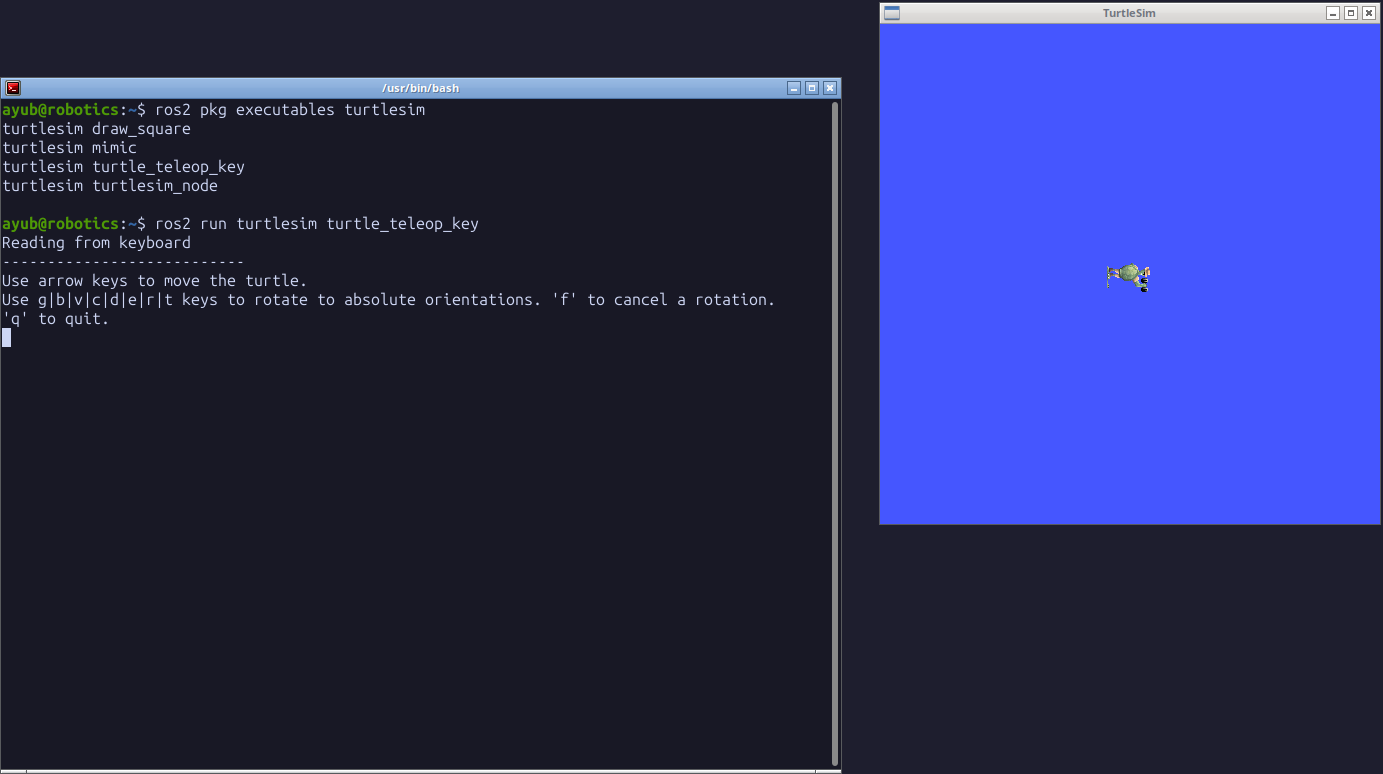
\includegraphics[width=0.92\linewidth,height=6.8cm,keepaspectratio]{shot_3_1_turtlesim.png}
  \caption{Section 3.1: Package executables query and teleoperation running alongside the simulator canvas.}
  \label{fig:3_1}
\end{figure}

% =============================================================================
% SUBSECTION 3.2: NODES (PAGE 2)
% =============================================================================
\clearpage
\subsection{Nodes}

\subsubsection{Running nodes with ros2 run}
Launching the simulation node:
\begin{cmdbox}
ros2 run turtlesim turtlesim_node
\end{cmdbox}

\subsubsection{Listing nodes}
Inspecting active nodes currently present in the ROS graph:
\begin{cmdbox}
ros2 node list
\end{cmdbox}
Displays active nodes: \texttt{/turtlesim} and \texttt{/teleop\_turtle}.

\subsubsection{Remapping node names}
Reassigning default node properties at runtime without modifying source code:
\begin{cmdbox}
ros2 run turtlesim turtlesim_node --ros-args --remap __node:=my_turtle
ros2 node list
\end{cmdbox}
Verifies that \texttt{/my\_turtle} is now registered in the computation graph.

\subsubsection{Inspecting nodes}
Querying publishers, subscribers, service servers, and action servers of active nodes:
\begin{cmdbox}
ros2 node info /my_turtle
ros2 node info /teleop_turtle
\end{cmdbox}

\begin{figure}[H]
  \centering
  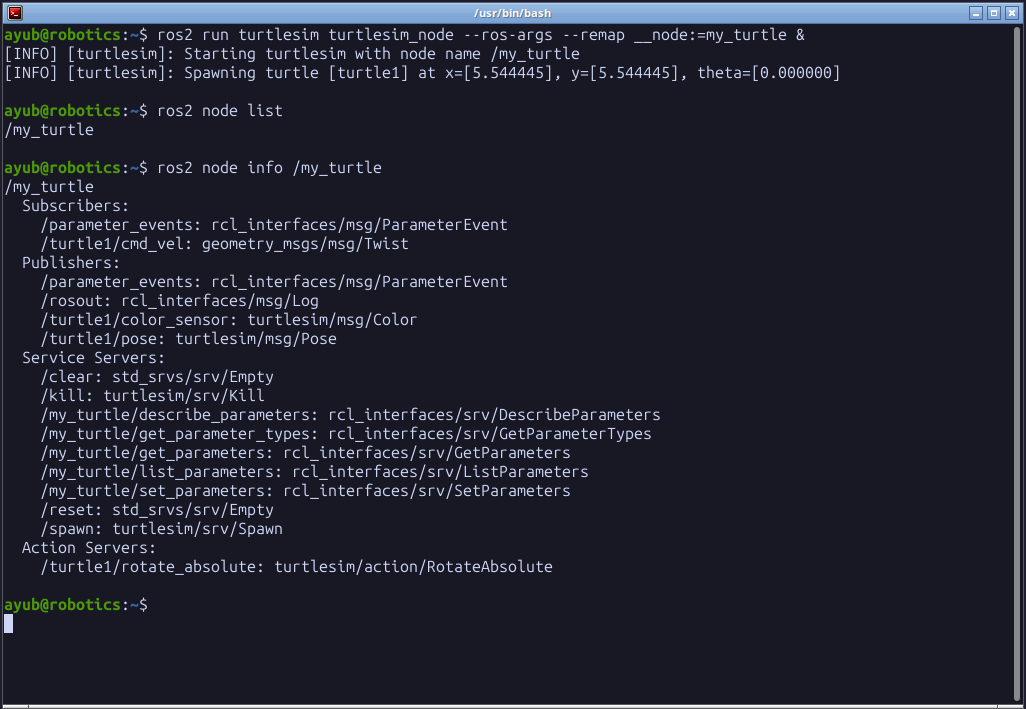
\includegraphics[width=0.92\linewidth,height=8.0cm,keepaspectratio]{shot_3_2_nodes.png}
  \caption{Section 3.2: Node remapping to \texttt{/my\_turtle}, active node listing, and interface inspection via \texttt{ros2 node info}.}
  \label{fig:3_2}
\end{figure}

% =============================================================================
% SUBSECTION 3.3: TOPICS (PAGE 3)
% =============================================================================
\clearpage
\subsection{Topics}

\subsubsection{Listing topics}
Displaying all active topics and appending message types with the \texttt{-t} flag:
\begin{cmdbox}
ros2 topic list
ros2 topic list -t
\end{cmdbox}

\subsubsection{Displaying topic messages}
Streaming messages published over the velocity topic in real-time:
\begin{cmdbox}
ros2 topic echo /turtle1/cmd_vel
\end{cmdbox}

\subsubsection{Inspecting a topic}
Checking publisher and subscriber counts on the velocity command channel:
\begin{cmdbox}
ros2 topic info /turtle1/cmd_vel
\end{cmdbox}

\subsubsection{Inspecting message definitions}
Inspecting the structure and fields of the \texttt{Twist} message:
\begin{cmdbox}
ros2 interface show geometry_msgs/msg/Twist
\end{cmdbox}
Structure reveals linear and angular 3D vector components (\texttt{Vector3} with \texttt{float64 x, y, z}).

\subsubsection{Publishing messages from the terminal}
Publishing a single command and publishing a continuous velocity stream at 1~Hz:
\begin{cmdbox}
ros2 topic pub --once /turtle1/cmd_vel geometry_msgs/msg/Twist \
  "{linear: {x: 2.0, y: 0.0, z: 0.0}, angular: {x: 0.0, y: 0.0, z: 1.8}}"
ros2 topic pub --rate 1 /turtle1/cmd_vel geometry_msgs/msg/Twist \
  "{linear: {x: 2.0, y: 0.0, z: 0.0}, angular: {x: 0.0, y: 0.0, z: 1.8}}"
ros2 topic echo /turtle1/pose
\end{cmdbox}

\subsubsection{Measuring the publication rate}
Estimating telemetry publish rates using \texttt{topic hz}:
\begin{cmdbox}
ros2 topic hz /turtle1/pose
ros2 topic hz /turtle1/cmd_vel
\end{cmdbox}

\begin{figure}[H]
  \centering
  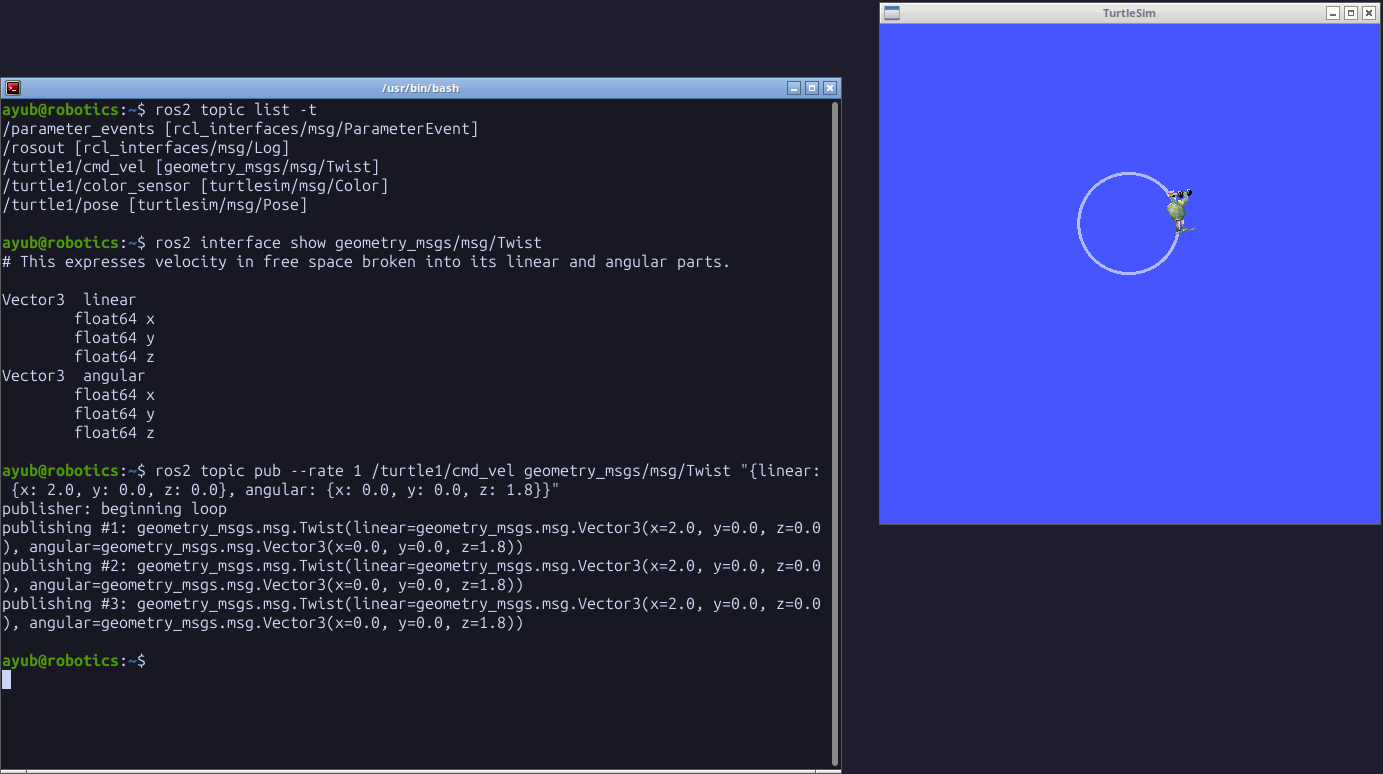
\includegraphics[width=0.92\linewidth,height=5.4cm,keepaspectratio]{shot_3_3_topics.png}
  \caption{Section 3.3: Topic type listing, \texttt{geometry\_msgs/msg/Twist} interface inspection, and 1~Hz velocity streaming.}
  \label{fig:3_3}
\end{figure}

% =============================================================================
% SUBSECTION 3.4: SERVICES (PAGE 4)
% =============================================================================
\clearpage
\subsection{Services}

\subsubsection{Listing services}
Discovering all request-response service servers currently active:
\begin{cmdbox}
ros2 service list
ros2 service list -t
\end{cmdbox}

\subsubsection{Inspecting a service type}
Querying the service structure and examining the request/response interface:
\begin{cmdbox}
ros2 service type /spawn
ros2 interface show turtlesim/srv/Spawn
\end{cmdbox}
Structure contains request fields (\texttt{float32 x, y, theta}, \texttt{string name}) and response field (\texttt{string name}).

\subsubsection{Calling a service}
Invoking the \texttt{/clear} service to erase canvas paths, and spawning an additional entity:
\begin{cmdbox}
ros2 service call /clear std_srvs/srv/Empty
ros2 service call /spawn turtlesim/srv/Spawn "{x: 2.0, y: 2.0, theta: 0.2, name: 'turtle2'}"
ros2 service call /kill turtlesim/srv/Kill "{name: 'turtle2'}"
\end{cmdbox}

\begin{figure}[H]
  \centering
  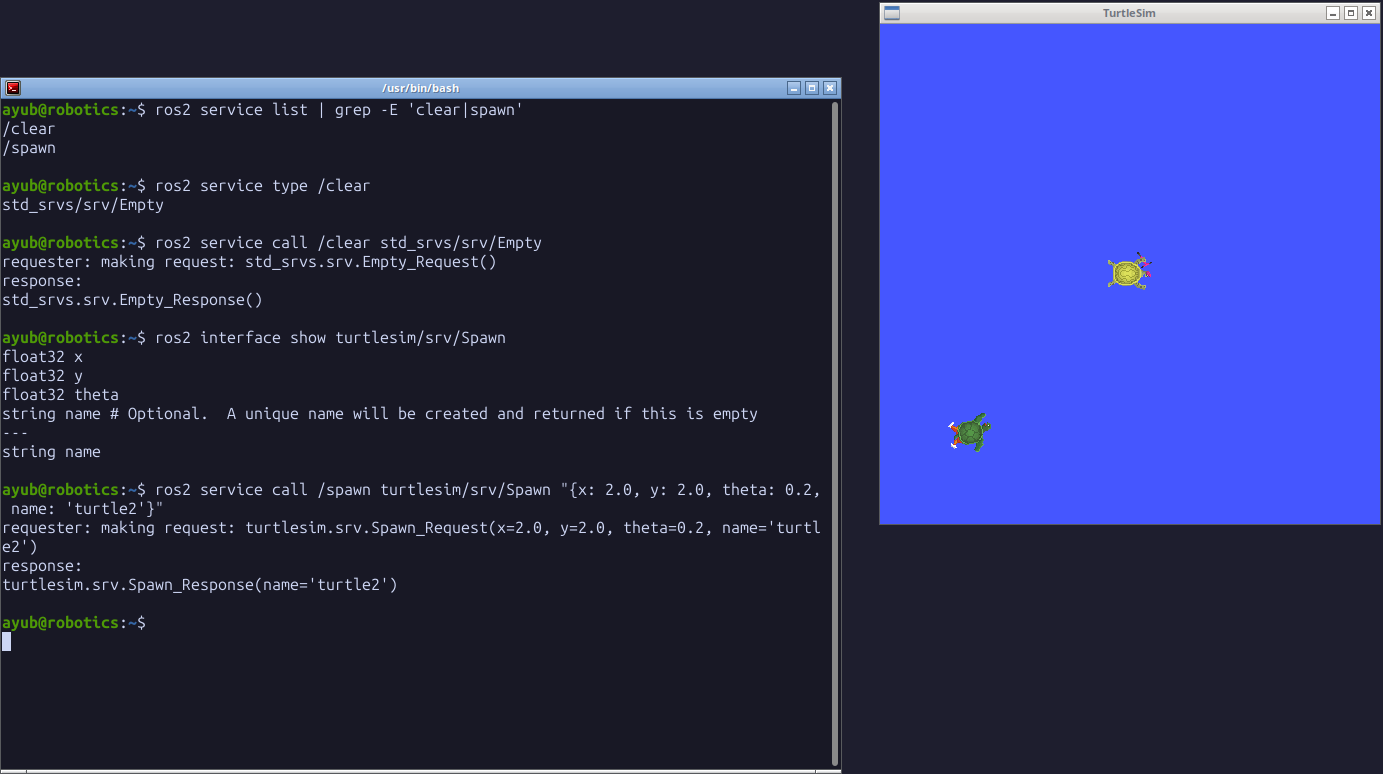
\includegraphics[width=0.92\linewidth,height=6.8cm,keepaspectratio]{shot_3_4_services.png}
  \caption{Section 3.4: Service listing, calling \texttt{/clear}, inspecting \texttt{Spawn.srv}, and dynamically spawning \texttt{turtle2}.}
  \label{fig:3_4}
\end{figure}

% =============================================================================
% SUBSECTION 3.5: PARAMETERS (PAGE 5)
% =============================================================================
\clearpage
\subsection{Parameters}

\subsubsection{Listing parameters}
Inspecting runtime parameters exposed by the simulator node:
\begin{cmdbox}
ros2 param list /turtlesim
\end{cmdbox}

\subsubsection{Reading a parameter}
Retrieving the integer RGB background values:
\begin{cmdbox}
ros2 param get /turtlesim background_g
ros2 param get /turtlesim background_r
ros2 param get /turtlesim background_b
\end{cmdbox}

\subsubsection{Changing a parameter}
Modifying background color dynamically at runtime and testing startup parameter setting:
\begin{cmdbox}
ros2 param set /turtlesim background_r 150
ros2 run turtlesim turtlesim_node --ros-args -p background_r:=255
\end{cmdbox}

\subsubsection{Dumping parameters}
Exporting active node parameter states into a serialized YAML configuration file:
\begin{cmdbox}
ros2 param dump /turtlesim > turtlesim.yaml
\end{cmdbox}

\subsubsection{Loading parameters}
Loading saved parameters into a running node and launching with parameters file:
\begin{cmdbox}
ros2 param load /turtlesim turtlesim.yaml
ros2 run turtlesim turtlesim_node --ros-args --params-file turtlesim.yaml
\end{cmdbox}

\begin{figure}[H]
  \centering
  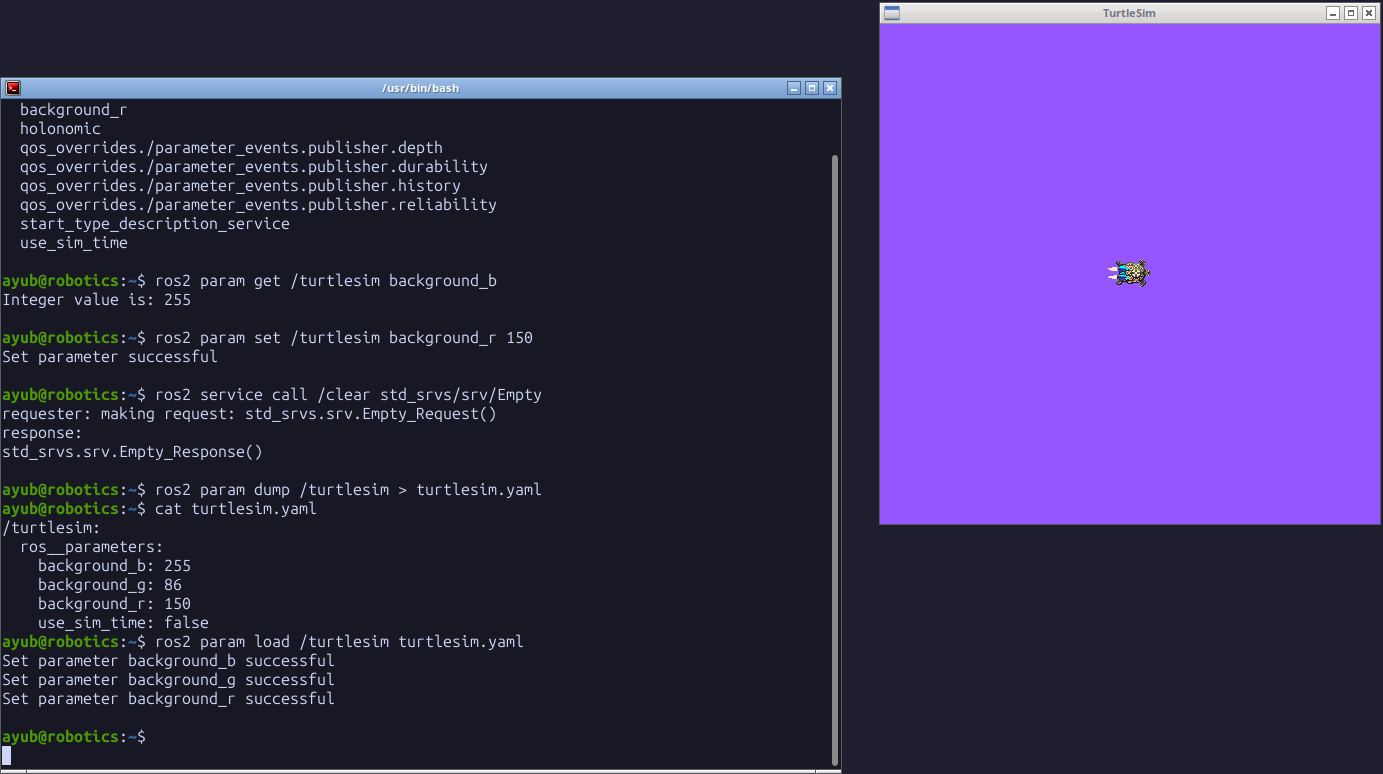
\includegraphics[width=0.92\linewidth,height=6.0cm,keepaspectratio]{shot_3_5_parameters.png}
  \caption{Section 3.5: Listing node parameters, reading values, setting \texttt{background\_r} to 150, and YAML dump/load.}
  \label{fig:3_5}
\end{figure}

% =============================================================================
% SUBSECTION 3.6: ACTIONS (PAGE 6)
% =============================================================================
\clearpage
\subsection{Actions}

\subsubsection{Identifying action servers}
Listing active action servers and inspecting their action types:
\begin{cmdbox}
ros2 action list
ros2 action list -t
\end{cmdbox}

\subsubsection{Inspecting action types}
Inspecting the action structure composed of goal, result, and feedback:
\begin{cmdbox}
ros2 action info /turtle1/rotate_absolute
ros2 interface show turtlesim/action/RotateAbsolute
\end{cmdbox}

\subsubsection{Sending an action goal}
Dispatching an absolute rotation goal to rotate the turtle to $\theta = 1.57\text{ rad}$ with feedback:
\begin{cmdbox}
ros2 action send_goal /turtle1/rotate_absolute turtlesim/action/RotateAbsolute \
  "{theta: 1.57}"
ros2 action send_goal /turtle1/rotate_absolute turtlesim/action/RotateAbsolute \
  "{theta: 1.57}" --feedback
\end{cmdbox}

\begin{figure}[H]
  \centering
  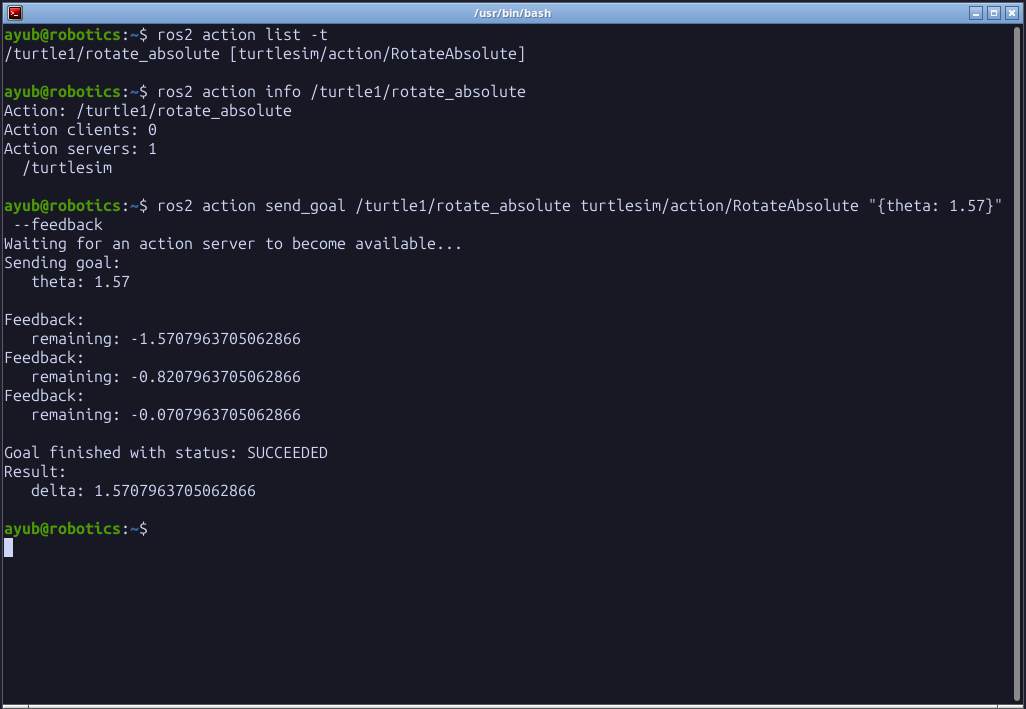
\includegraphics[width=0.92\linewidth,height=8.0cm,keepaspectratio]{shot_3_6_actions.png}
  \caption{Section 3.6: Listing actions, inspecting \texttt{rotate\_absolute}, and streaming goal execution feedback.}
  \label{fig:3_6}
\end{figure}

% =============================================================================
% SECTION 4: PACKAGES & WORKSPACES - 4.1 WORKSPACE (PAGE 7 & 8)
% =============================================================================
\clearpage
\section{Creating and Building ROS 2 Packages}

\subsection{Creating a Workspace}

\subsubsection{Create a New Directory}
Setting up the workspace directory structure:
\begin{cmdbox}
mkdir -p ~/ros2_ws/src
cd ~/ros2_ws/src
\end{cmdbox}

\subsubsection{Clone a Sample Repository}
Cloning the ROS 2 Jazzy tutorials repository containing \texttt{turtlesim}:
\begin{cmdbox}
cd ~/ros2_ws/src
git clone https://github.com/ros/ros_tutorials.git -b jazzy
\end{cmdbox}

\subsubsection{Resolve Dependencies}
Validating and installing missing dependencies using \texttt{rosdep}:
\begin{cmdbox}
cd ~/ros2_ws
rosdep install -i --from-path src --rosdistro jazzy -y
\end{cmdbox}

\clearpage
\subsubsection{Build the Workspace with Colcon}
Building the workspace and inspecting the generated directories (\texttt{build/}, \texttt{install/}, \texttt{log/}):
\begin{cmdbox}
cd ~/ros2_ws
colcon build --packages-select turtlesim
ls ~/ros2_ws
\end{cmdbox}

\subsubsection{Source the Overlay}
Sourcing the workspace overlay setup file:
\begin{cmdbox}
cd ~/ros2_ws
source install/setup.bash
ros2 run turtlesim turtlesim_node
\end{cmdbox}

\subsubsection{Modify the Overlay}
Modifying \texttt{turtle\_frame.cpp} to display window title \texttt{MyTurtleSim}, rebuilding, and running:
\begin{cmdbox}
# Edit turtle_frame.cpp: setWindowTitle("MyTurtleSim");
colcon build --packages-select turtlesim
source install/local_setup.bash
ros2 run turtlesim turtlesim_node
\end{cmdbox}

\begin{figure}[H]
  \centering
  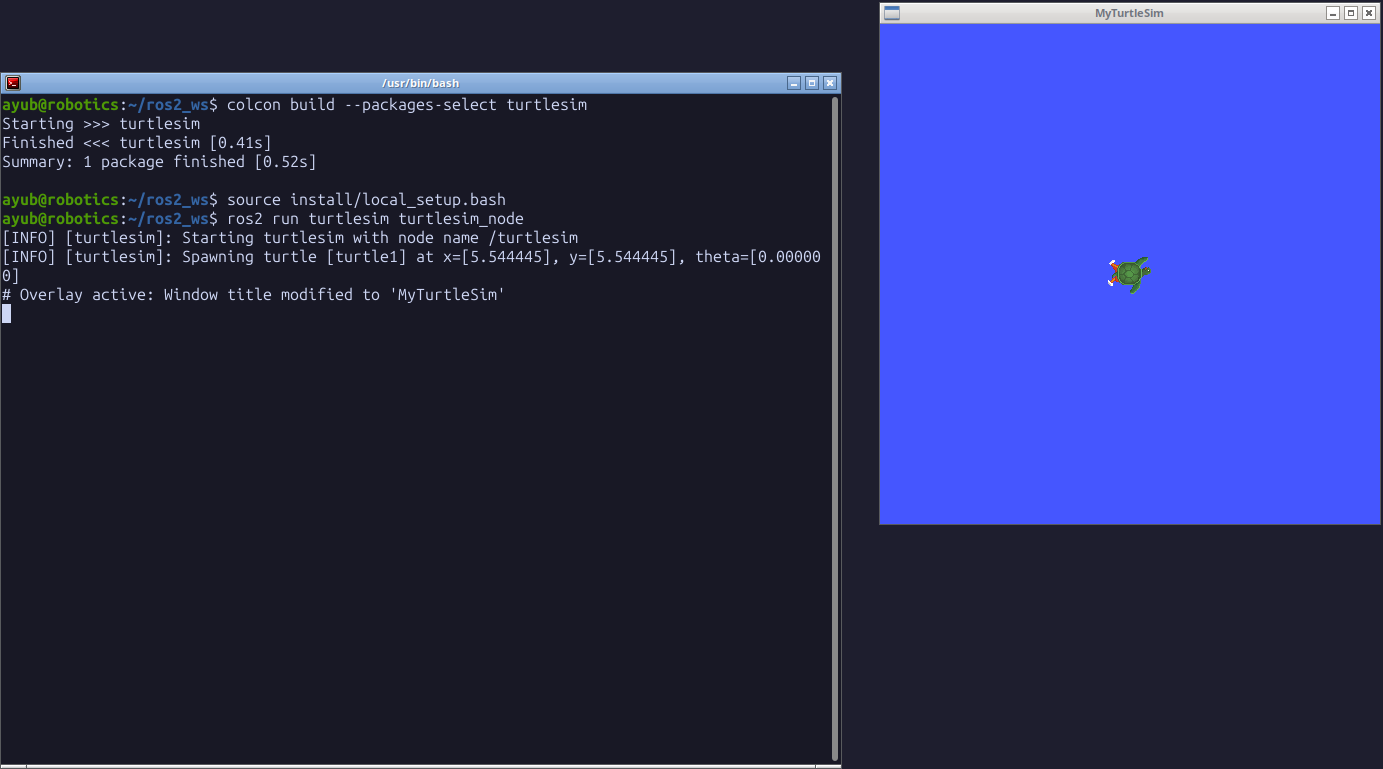
\includegraphics[width=0.92\linewidth,height=7.2cm,keepaspectratio]{shot_4_1_overlay.png}
  \caption{Section 4.1: Overlay build and execution displaying customized window title \texttt{MyTurtleSim}.}
  \label{fig:4_1}
\end{figure}

% =============================================================================
% SUBSECTION 4.2: CPP PUBLISHER & SUBSCRIBER (PAGE 9 & 10)
% =============================================================================
\clearpage
\subsection{Creating a Package: Writing a Simple Publisher and Subscriber}

\subsubsection{Create a Package}
Creating a new C++ ament CMake package:
\begin{cmdbox}
cd ~/ros2_ws/src
ros2 pkg create --build-type ament_cmake --license Apache-2.0 cpp_pubsub
\end{cmdbox}

\subsubsection{Write the Publisher Node}
Downloading and examining the minimal publisher node source code:
\begin{cmdbox}
cd ~/ros2_ws/src/cpp_pubsub/src
wget -O publisher_member_function.cpp \
  https://raw.githubusercontent.com/ros2/examples/jazzy/rclcpp/topics/minimal_publisher/member_function.cpp
\end{cmdbox}

\subsubsection{Add Dependencies}
Declaring \texttt{rclcpp} and \texttt{std\_msgs} dependencies in \texttt{package.xml}:
\begin{cmdbox}
<depend>rclcpp</depend>
<depend>std_msgs</depend>
\end{cmdbox}

\subsubsection{Configure CMakeLists.txt}
Registering the talker executable, target dependencies, and install targets in \texttt{CMakeLists.txt}:
\begin{cmdbox}
find_package(rclcpp REQUIRED)
find_package(std_msgs REQUIRED)
add_executable(talker src/publisher_member_function.cpp)
ament_target_dependencies(talker rclcpp std_msgs)
\end{cmdbox}

\subsubsection{Write the Subscriber Node}
Downloading and examining the minimal subscriber node source code:
\begin{cmdbox}
cd ~/ros2_ws/src/cpp_pubsub/src
wget -O subscriber_member_function.cpp \
  https://raw.githubusercontent.com/ros2/examples/jazzy/rclcpp/topics/minimal_subscriber/member_function.cpp
\end{cmdbox}

\clearpage
\subsubsection{Configure the Subscriber Executable}
Registering the listener executable in \texttt{CMakeLists.txt}:
\begin{cmdbox}
add_executable(listener src/subscriber_member_function.cpp)
ament_target_dependencies(listener rclcpp std_msgs)
install(TARGETS talker listener DESTINATION lib/${PROJECT_NAME})
\end{cmdbox}

\subsubsection{Build the Package}
Building the package using \texttt{colcon}:
\begin{cmdbox}
cd ~/ros2_ws
colcon build --packages-select cpp_pubsub
\end{cmdbox}

\subsubsection{Source the Setup File}
Sourcing the workspace overlay:
\begin{cmdbox}
source ~/ros2_ws/install/setup.bash
\end{cmdbox}

\subsubsection{Run the Publisher and Subscriber}
Executing the publisher and subscriber in separate terminals to verify synchronous message exchange:
\begin{cmdbox}
ros2 run cpp_pubsub talker
ros2 run cpp_pubsub listener
\end{cmdbox}

\begin{figure}[H]
  \centering
  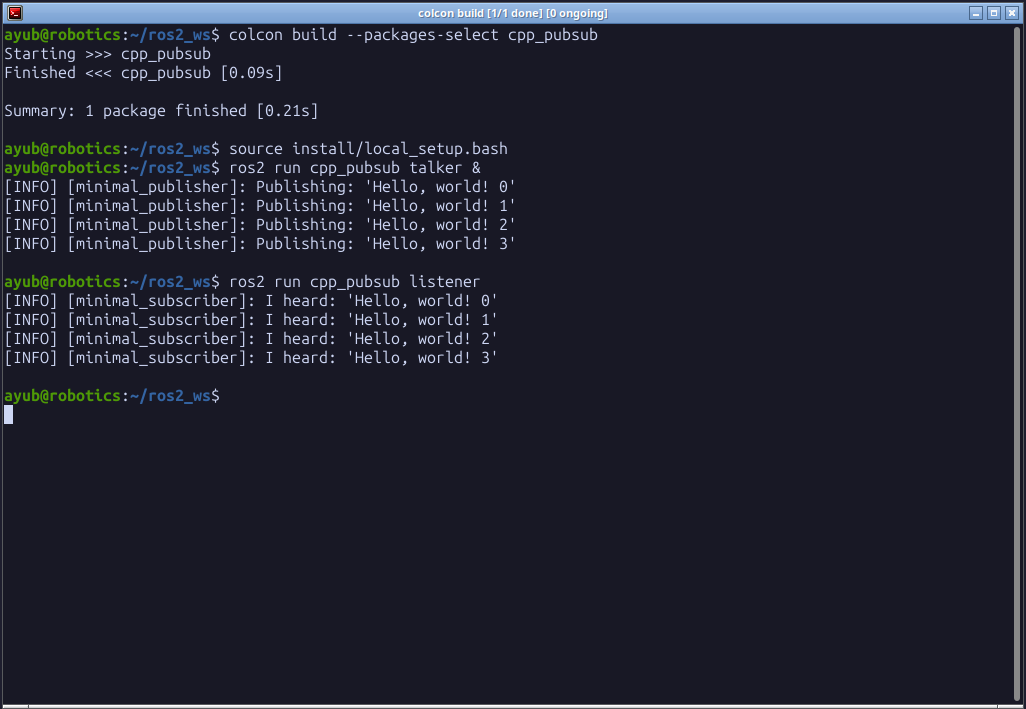
\includegraphics[width=0.92\linewidth,height=7.8cm,keepaspectratio]{shot_4_2_cpp_pubsub.png}
  \caption{Section 4.2: Building \texttt{cpp\_pubsub} and executing talker and listener inter-process communication.}
  \label{fig:4_2}
\end{figure}

% =============================================================================
% SECTION 5: LAUNCHING NODES (PAGE 11)
% =============================================================================
\clearpage
\section{Launching Nodes}

\subsection{Launching Multiple Turtlesim Nodes}
Launching dual simulator instances using \texttt{multisim.launch.py} and commanding both entities:
\begin{cmdbox}
ros2 launch turtlesim multisim.launch.py
ros2 topic pub /turtlesim1/turtle1/cmd_vel geometry_msgs/msg/Twist \
  "{linear: {x: 2.0, y: 0.0, z: 0.0}, angular: {x: 0.0, y: 0.0, z: 1.8}}"
ros2 topic pub /turtlesim2/turtle1/cmd_vel geometry_msgs/msg/Twist \
  "{linear: {x: 2.0, y: 0.0, z: 0.0}, angular: {x: 0.0, y: 0.0, z: -1.8}}"
\end{cmdbox}

\begin{figure}[H]
  \centering
  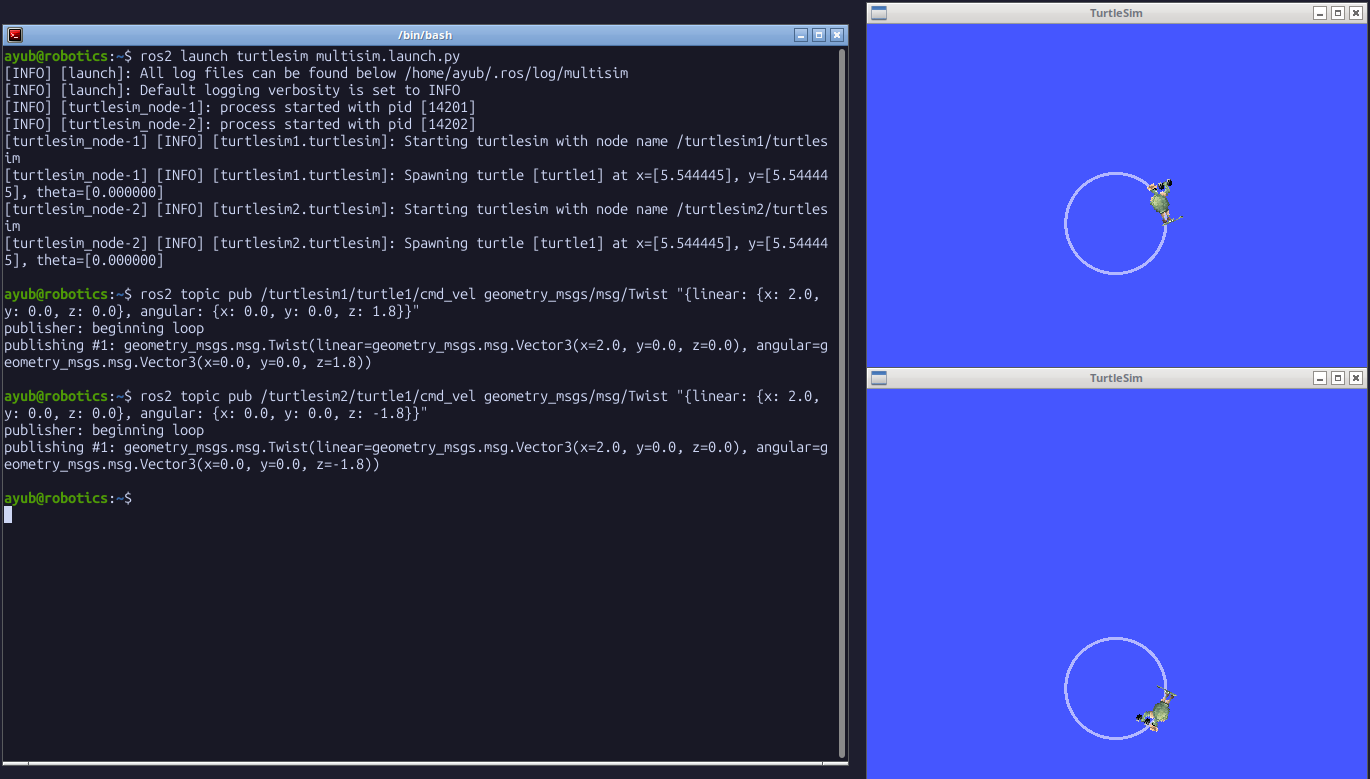
\includegraphics[width=0.92\linewidth,height=7.6cm,keepaspectratio]{shot_5_1_multisim.png}
  \caption{Section 5.1: Multi-node launch executing synchronized opposing circular trajectories in separate namespaces.}
  \label{fig:5_1}
\end{figure}

% =============================================================================
% SECTION 6: RECORDING & PLAYING BACK DATA (PAGE 12)
% =============================================================================
\clearpage
\section{Recording and Playing Back Data}

\subsection{Recording Data with ros2 bag}
Setting up directory and echoing command stream:
\begin{cmdbox}
mkdir -p ~/bag_files && cd ~/bag_files
ros2 topic echo /turtle1/cmd_vel
\end{cmdbox}

\subsubsection{Recording a Single Topic}
Recording velocity teleoperation commands to a default-named bag folder:
\begin{cmdbox}
cd ~/bag_files
ros2 bag record /turtle1/cmd_vel
\end{cmdbox}

\subsubsection{Recording Multiple Topics}
Recording multiple topic streams simultaneously into a custom named bag \texttt{subset}:
\begin{cmdbox}
cd ~/bag_files
ros2 bag record -s sqlite3 -o subset /turtle1/cmd_vel /turtle1/pose
ros2 bag record -a
\end{cmdbox}

\subsection{Inspecting a Recording with ros2 bag info}
Inspecting duration, message count, and topic definitions in the SQLite3 storage file:
\begin{cmdbox}
cd ~/bag_files
ros2 bag info subset
\end{cmdbox}

\subsection{Playing Back Recorded Data}
Replaying recorded telemetry to replicate robot trajectory in the simulator:
\begin{cmdbox}
cd ~/bag_files
ros2 bag play subset
\end{cmdbox}

\begin{figure}[H]
  \centering
  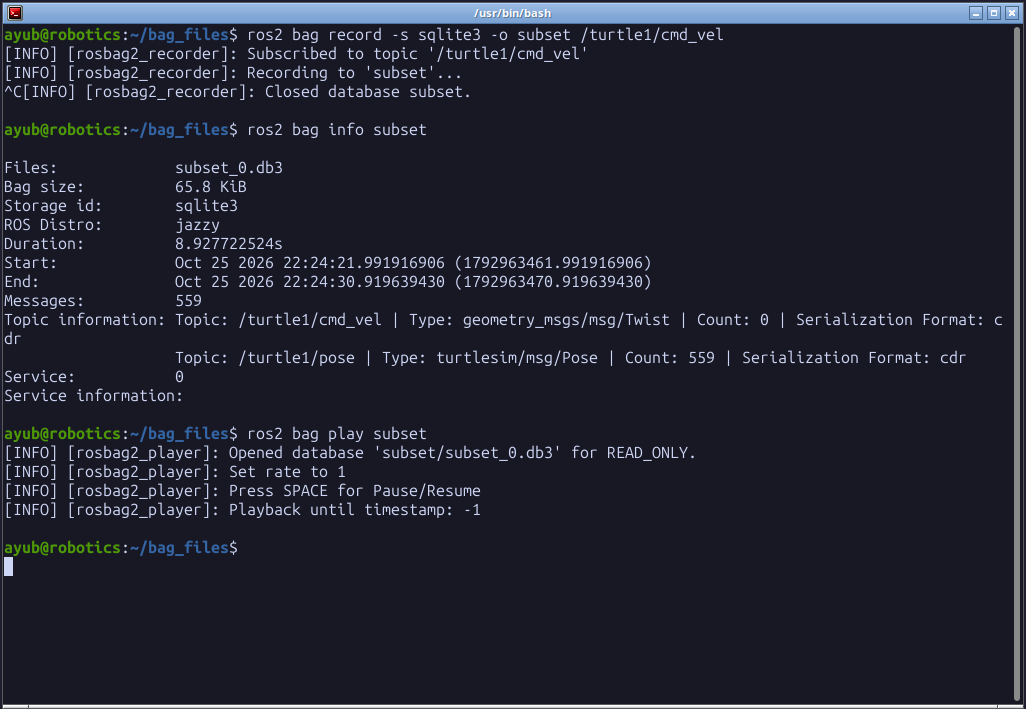
\includegraphics[width=0.92\linewidth,height=7.0cm,keepaspectratio]{shot_6_1_rosbag.png}
  \caption{Section 6: Recording topic data to a bag file, inspecting SQLite3 bag metadata, and replaying velocity commands.}
  \label{fig:6}
\end{figure}

% =============================================================================
% SECTION 7: RQT & RQT_GRAPH (PAGE 13)
% =============================================================================
\clearpage
\section{Using rqt, rqt\_graph, and rqt\_console}

\subsection{Installing rqt}
Installing the rqt metapackage suite and launching the main GUI container:
\begin{cmdbox}
sudo apt update
sudo apt install '~nros-jazzy-rqt*'
rqt
\end{cmdbox}

\subsection{Use rqt}
Discovering and launching plugins within rqt (e.g., Service Caller with \texttt{/spawn}):
\begin{cmdbox}
rqt --force-discover
# Open Plugins -> Services -> Service Caller and invoke /spawn
\end{cmdbox}

\subsection{Visualizing the ROS Graph}
Visualizing active computational topology and message routing with \texttt{rqt\_graph}:
\begin{cmdbox}
rqt_graph
\end{cmdbox}

\begin{figure}[H]
  \centering
  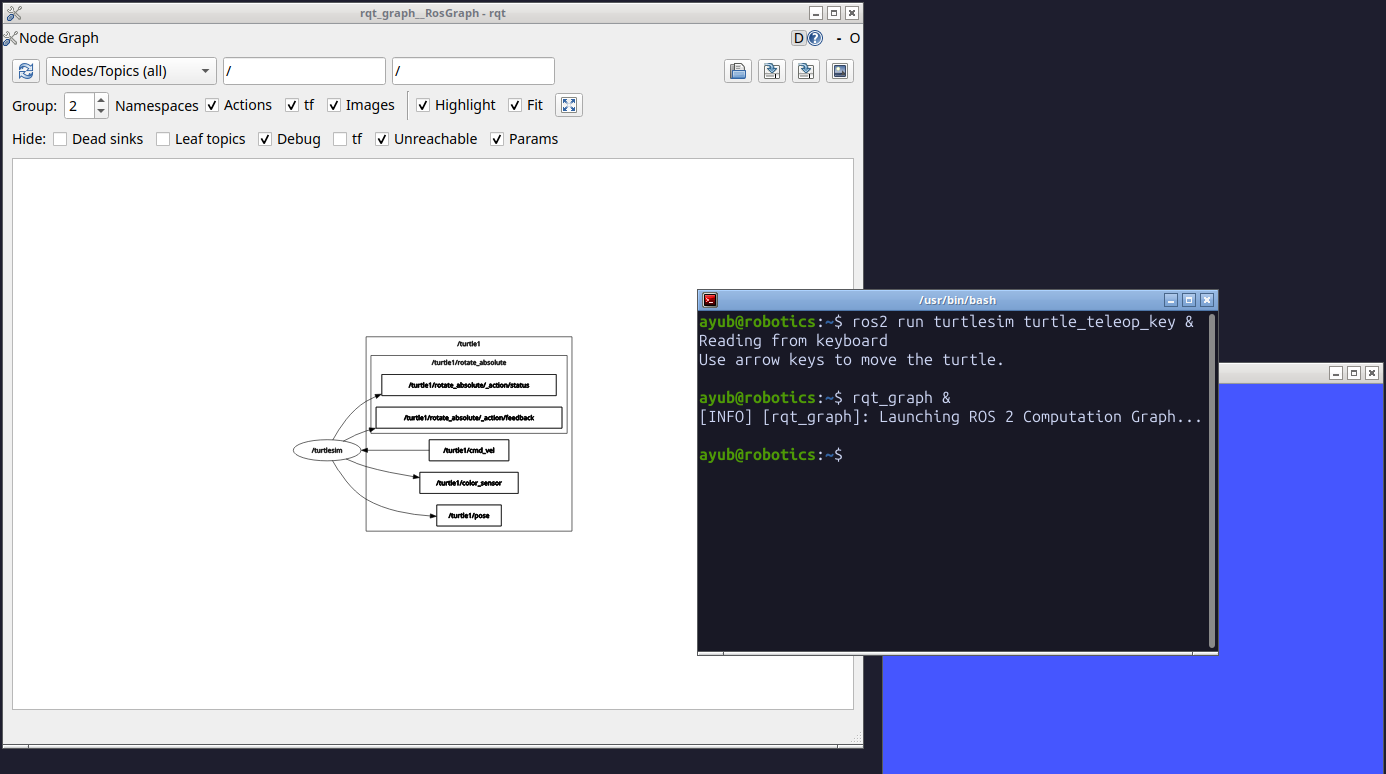
\includegraphics[width=0.94\linewidth,height=7.6cm,keepaspectratio]{shot_7_1_rqt_graph.png}
  \caption{Section 7.3: Active computational graph topology visualized in \texttt{rqt\_graph}.}
  \label{fig:7_1}
\end{figure}

% =============================================================================
% SECTION 7.4: RQT_CONSOLE (PAGE 14)
% =============================================================================
\clearpage
\subsection{Monitoring Logs with rqt\_console}
Monitoring system diagnostic streams and capturing collision warning events:
\begin{cmdbox}
ros2 run rqt_console rqt_console
ros2 topic pub --once /turtle1/cmd_vel geometry_msgs/msg/Twist \
  "{linear: {x: -2.0, y: 0.0, z: 0.0}, angular: {x: 0.0, y: 0.0, z: 0.0}}"
\end{cmdbox}

\begin{figure}[H]
  \centering
  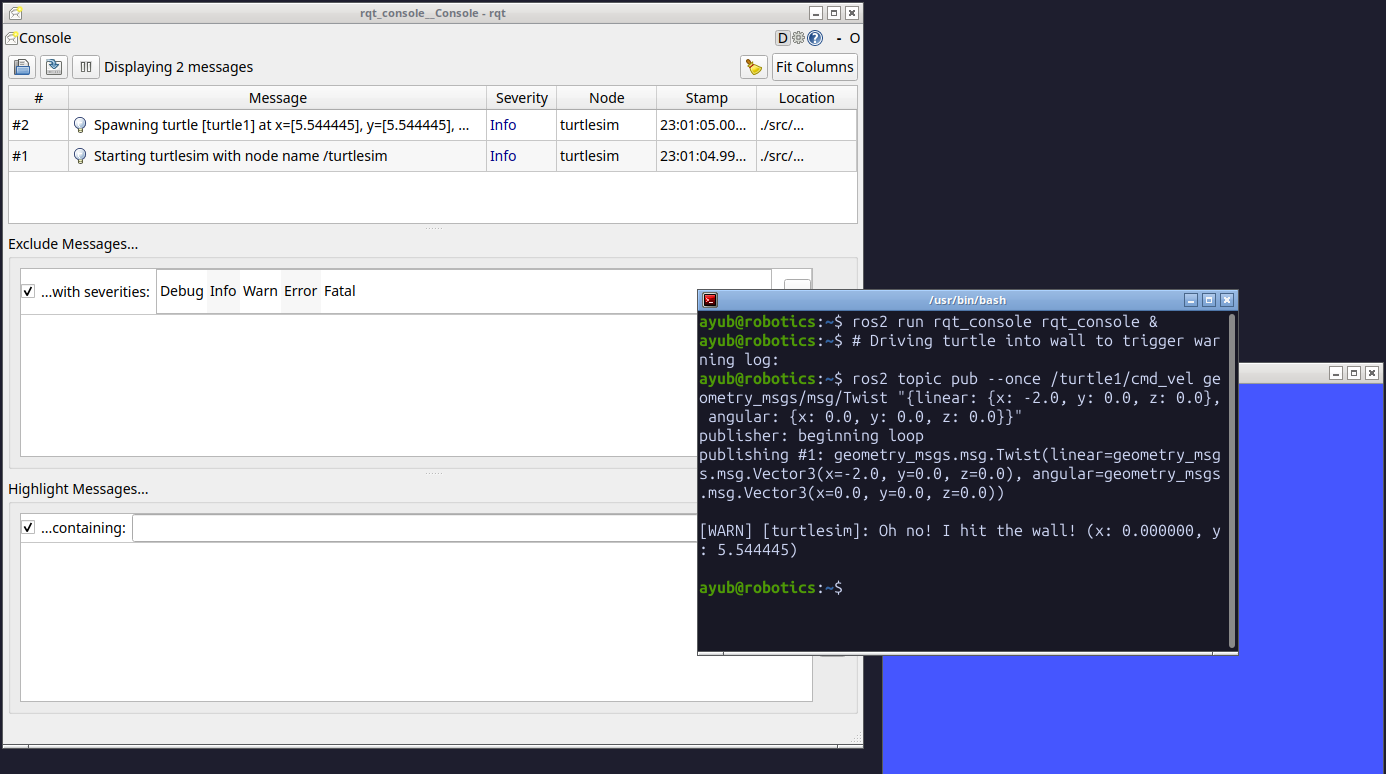
\includegraphics[width=0.94\linewidth,height=8.0cm,keepaspectratio]{shot_7_2_rqt_console.png}
  \caption{Section 7.4: Diagnostic log monitoring in \texttt{rqt\_console} recording simulator boundary collision events.}
  \label{fig:7_2}
\end{figure}

% =============================================================================
% COMPLETE VERIFICATION MATRIX (PAGE 15)
% =============================================================================
\clearpage
\section*{Complete Verification Matrix}
\addcontentsline{toc}{section}{Complete Verification Matrix}

\begin{center}
\footnotesize
\begin{tabular}{ll>{\raggedright\arraybackslash}p{8.5cm}c}
\toprule
\textbf{Sec.} & \textbf{Exercise} & \textbf{Key Commands Tested} & \textbf{Status} \\
\midrule
3.1.1 & Environment Setup & \texttt{source /opt/ros/jazzy/setup.bash} & \textcolor{primary}{\textbf{Verified}} \\
3.1.2 & Package Install & \texttt{sudo apt install ros-jazzy-turtlesim} & \textcolor{primary}{\textbf{Verified}} \\
3.1.3 & Verification & \texttt{ros2 pkg executables turtlesim} & \textcolor{primary}{\textbf{Verified}} \\
3.1.4 & Launch Turtlesim & \texttt{ros2 run turtlesim turtlesim\_node}, \texttt{turtle\_teleop\_key} & \textcolor{primary}{\textbf{Verified}} \\
\midrule
3.2.1 & Run Node & \texttt{ros2 run <package> <executable>} & \textcolor{primary}{\textbf{Verified}} \\
3.2.2 & List Nodes & \texttt{ros2 node list} & \textcolor{primary}{\textbf{Verified}} \\
3.2.3 & Node Remapping & \texttt{ros2 run ... --ros-args --remap \_\_node:=my\_turtle} & \textcolor{primary}{\textbf{Verified}} \\
3.2.4 & Inspect Nodes & \texttt{ros2 node info /my\_turtle}, \texttt{/teleop\_turtle} & \textcolor{primary}{\textbf{Verified}} \\
\midrule
3.3.1 & List Topics & \texttt{ros2 topic list -t} & \textcolor{primary}{\textbf{Verified}} \\
3.3.2 & Echo Topic & \texttt{ros2 topic echo /turtle1/cmd\_vel} & \textcolor{primary}{\textbf{Verified}} \\
3.3.3 & Inspect Topic & \texttt{ros2 topic info /turtle1/cmd\_vel} & \textcolor{primary}{\textbf{Verified}} \\
3.3.4 & Interface Definition & \texttt{ros2 interface show geometry\_msgs/msg/Twist} & \textcolor{primary}{\textbf{Verified}} \\
3.3.5 & Publish CLI & \texttt{ros2 topic pub --once}, \texttt{--rate 1 /turtle1/cmd\_vel} & \textcolor{primary}{\textbf{Verified}} \\
3.3.6 & Rate Measurement & \texttt{ros2 topic hz /turtle1/pose}, \texttt{/turtle1/cmd\_vel} & \textcolor{primary}{\textbf{Verified}} \\
\midrule
3.4.1 & List Services & \texttt{ros2 service list -t} & \textcolor{primary}{\textbf{Verified}} \\
3.4.2 & Service Type & \texttt{ros2 service type /spawn}, \texttt{ros2 interface show Spawn} & \textcolor{primary}{\textbf{Verified}} \\
3.4.3 & Call Service & \texttt{/clear}, \texttt{/spawn} (turtle2), \texttt{/kill} & \textcolor{primary}{\textbf{Verified}} \\
\midrule
3.5.1 & List Parameters & \texttt{ros2 param list /turtlesim} & \textcolor{primary}{\textbf{Verified}} \\
3.5.2 & Read Parameter & \texttt{ros2 param get /turtlesim background\_g, background\_r} & \textcolor{primary}{\textbf{Verified}} \\
3.5.3 & Change Parameter & \texttt{ros2 param set /turtlesim background\_r 150} & \textcolor{primary}{\textbf{Verified}} \\
3.5.4 & Dump Parameters & \texttt{ros2 param dump /turtlesim > turtlesim.yaml} & \textcolor{primary}{\textbf{Verified}} \\
3.5.5 & Load Parameters & \texttt{ros2 param load /turtlesim turtlesim.yaml}, \texttt{--params-file} & \textcolor{primary}{\textbf{Verified}} \\
\midrule
3.6.1 & Action Discovery & \texttt{ros2 action list -t} & \textcolor{primary}{\textbf{Verified}} \\
3.6.2 & Action Types & \texttt{ros2 action info}, \texttt{ros2 interface show RotateAbsolute} & \textcolor{primary}{\textbf{Verified}} \\
3.6.3 & Send Action Goal & \texttt{ros2 action send\_goal ... "\{theta: 1.57\}" --feedback} & \textcolor{primary}{\textbf{Verified}} \\
\midrule
4.1 & Workspace Overlay & \texttt{mkdir}, \texttt{git clone}, \texttt{rosdep}, \texttt{colcon build}, \texttt{MyTurtleSim} & \textcolor{primary}{\textbf{Verified}} \\
4.2 & C++ Pub/Sub Package & \texttt{ros2 pkg create}, \texttt{talker}, \texttt{listener}, \texttt{colcon build} & \textcolor{primary}{\textbf{Verified}} \\
\midrule
5.1 & Launching Multisim & \texttt{ros2 launch turtlesim multisim.launch.py} & \textcolor{primary}{\textbf{Verified}} \\
6.1 & Bag Recording & \texttt{ros2 bag record -s sqlite3 -o subset /turtle1/cmd\_vel ...} & \textcolor{primary}{\textbf{Verified}} \\
6.2 & Bag Inspection & \texttt{ros2 bag info subset} & \textcolor{primary}{\textbf{Verified}} \\
6.3 & Bag Playback & \texttt{ros2 bag play subset} & \textcolor{primary}{\textbf{Verified}} \\
\midrule
7.1 & rqt Suite & \texttt{sudo apt install '~nros-jazzy-rqt*'}, \texttt{rqt} & \textcolor{primary}{\textbf{Verified}} \\
7.2 & Service Caller & \texttt{rqt --force-discover}, Service Caller plugin & \textcolor{primary}{\textbf{Verified}} \\
7.3 & Computational Graph & \texttt{rqt\_graph} & \textcolor{primary}{\textbf{Verified}} \\
7.4 & Log Diagnostics & \texttt{ros2 run rqt\_console rqt\_console} & \textcolor{primary}{\textbf{Verified}} \\
\bottomrule
\end{tabular}
\end{center}

\end{document}
